\section{Experiments}
\label{sec:experiments}
\subsection{Kernel Ridge Regression}
\begin{figure}
\centering
\begin{tabular}{c c}
	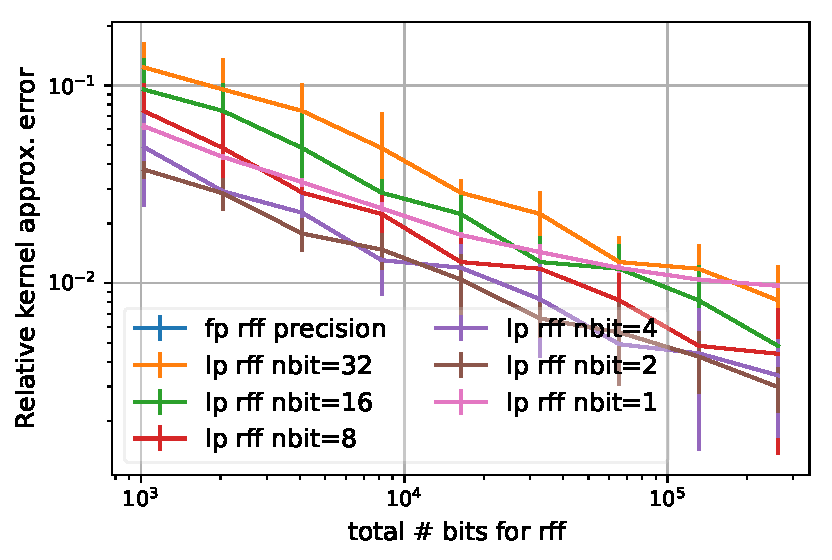
\includegraphics[width=.45\linewidth]{figures/kernel_approx_error.pdf} &
	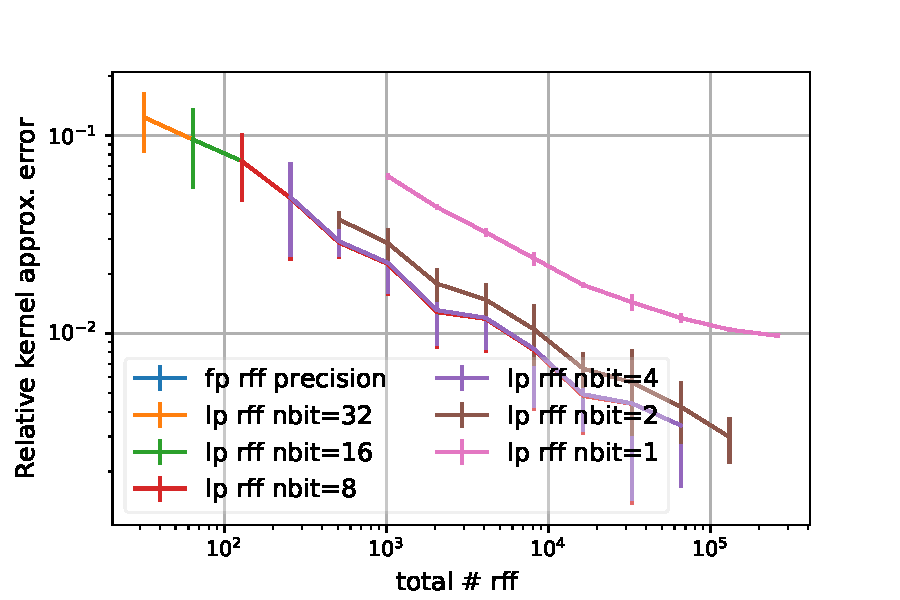
\includegraphics[width=.45\linewidth]{figures/kernel_approx_error_n_fp.pdf} \\
	(a) & (b) \\
	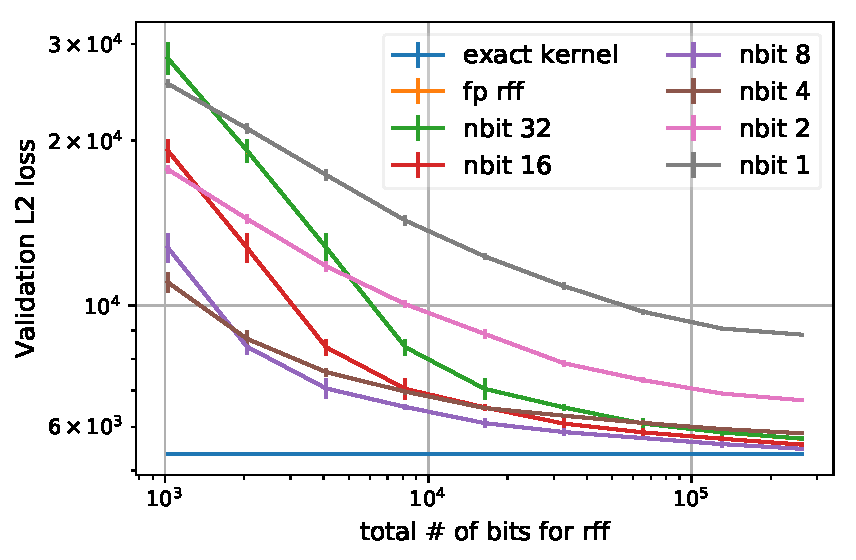
\includegraphics[width=.45\linewidth]{figures/valid_l2.pdf} &
	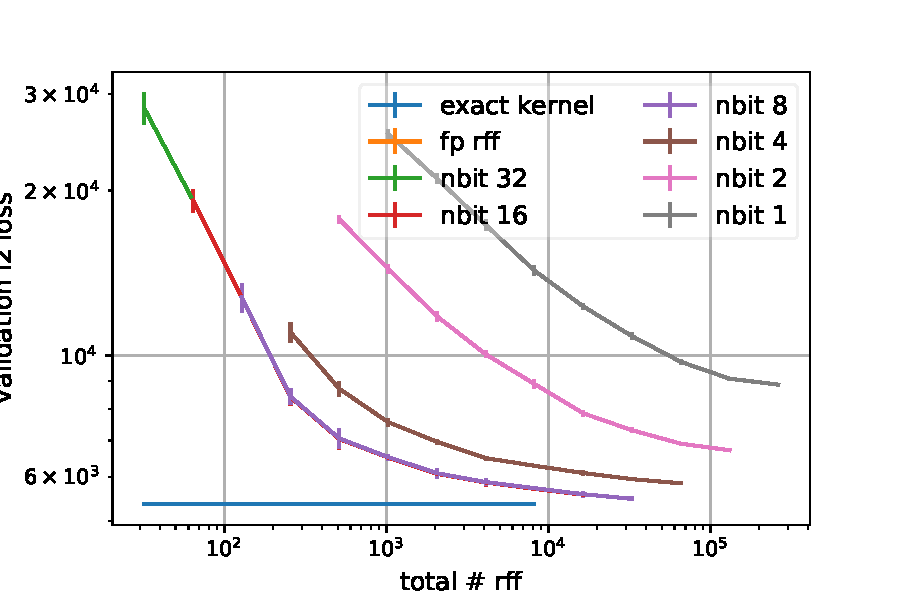
\includegraphics[width=.45\linewidth]{figures/valid_l2_n_fp.pdf}  \\
		(c) & (d) \\
\end{tabular}
\caption{Kernel approximation and validation L2 loss for Kernel Ridge Regression on UCI Census dataset. (a) and (b) compare different precision representation under same memory bits budgets. (c) and (d) compare different precision representation with the same number of random Fourier features.}
\label{fig:kernel_and_l2}
\end{figure}

We use UCI Census dataset for the experiments on kernel ridge regression. This dataset contains 16k training samples with 119 original features. Besides from reporting the kernel approximation errors, we also report the validation l2 loss in the regression problem. The reported l2 loss for each feature precision is from a grid search over $\{1e^{-6}, 1e^{-5}, ..., 1e^{-1}, 1, 10, 100\}$. To report statistically meaningful results, we average the performance metrics from 5 stochastic quantization using different random seeds. We uniformly use Gaussian kernels with $\sigma=30.0$ for our experiments on kernel ridge regression.

\subsubsection{Kernel approximation error and validation l2 loss}
As shown in Figure~\ref{fig:kernel_and_l2} (b) and (d), when using the same number of random Fourier features, the kernel approximation error and validation l2 loss only start to observably degrade after the the precision gets lower than 8 bits. For precision using 8 bits or higher number of bits, the validation l2 loss closely overlap with the ones from full precision random Fourier features. Further more, we compare the performance of feature representation in different precision under the same memory bits budget for each data sample. Kernel methods based on RFF typically improves when more RFF presents, while more precise feature representation can demonstrate lower approximation error. \emph{Indeed, under the memory budgets, we observe a trade-off between the number of RFF and the representation precision of RFF in~\ref{fig:kernel_and_l2}(a) and (b). Specifically, under different memory budget for the RFF representation of each data sample, 2 or 4 bits representation presents the best kernel approximation, while 8 bits demonstrates the best validation l2 loss consistently.}

%\begin{figure}
%	\centering
%	\begin{tabular}{c c}
%		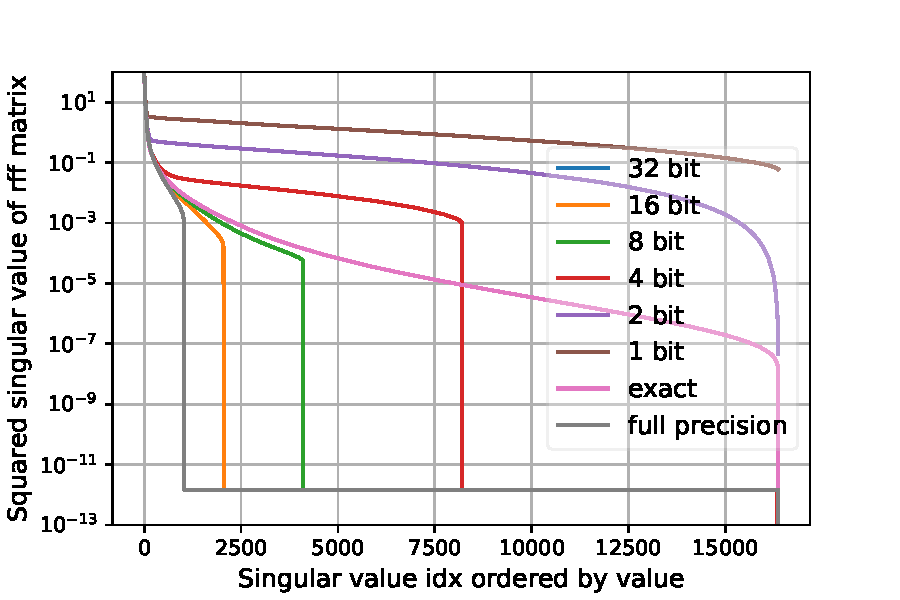
\includegraphics[width=.45\linewidth]{figures/spectrum_1024.pdf} &
%		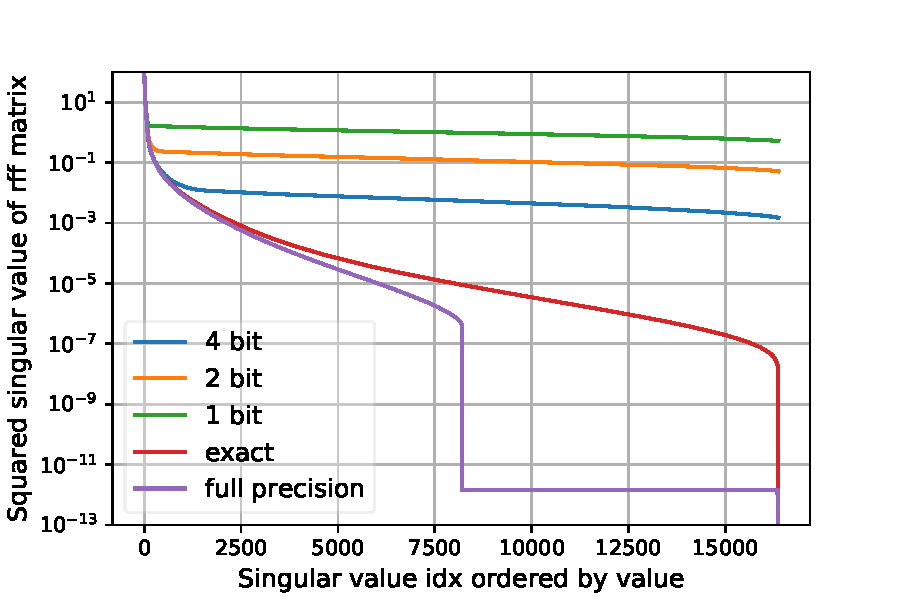
\includegraphics[width=.45\linewidth]{figures/spectrum_8192.pdf}  \\
%		(a) & (b) \\
%		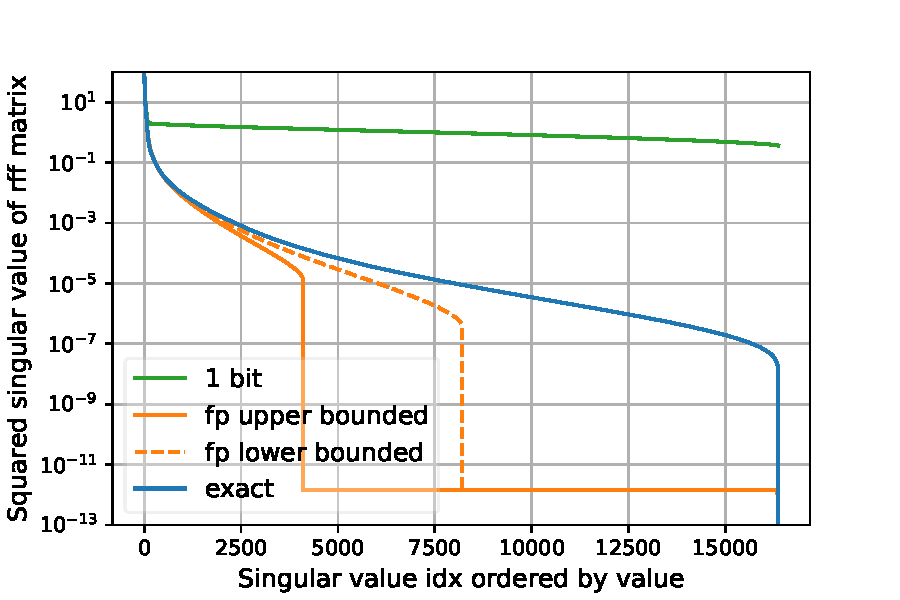
\includegraphics[width=.45\linewidth]{figures/different_spectrum_with_same_kernel_approx_error_log.pdf} &
%		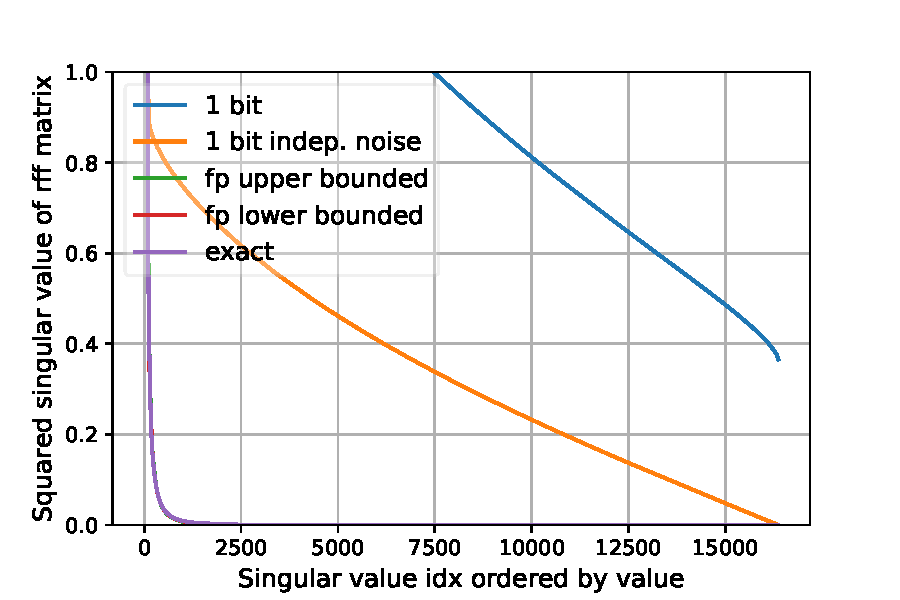
\includegraphics[width=.45\linewidth]{figures/different_spectrum_with_same_kernel_approx_error.pdf}\\
%		(c) & (d)
%	\end{tabular}
%	\caption{Spectrum (eigen values) of the kernel matrix. The spectrums from different precision representation are shown under a) 3.2k (equivalent to 1024 full precision rffs) and b) 25.6k bits memory budget (equivalent to 8192 full precision rffs) for the feature of each sample. (c) Configurations with similar approximation errors can demonstrate very different spectrum; we compare the 1 bit representation to the full precision configurations giving 1) the highest approx. error that is lower than the 1 bit configuration 2) the lowest approx. error that is higher than the 1bit configuration. (c) Replot (b) in decimal scale to visualize the difference of spectrums; the spectrums from kernel matrix using 1) a single stochastic quantization and 2) two independent stochastic quantization for the feature matrix and its transpose. \emph{Note in (c) and (d), we can observe independent quantization for RFF matrix and its transpose (indep. noise curves in the figures) presents spectrum closer to the exact kernel than using the same stochastic quantization for RFF matrix and its transpose.} }
%	\label{fig:spectrums}
%\end{figure}

\subsubsection{Spectrum of kernel matrix correlates with l2 loss}

\begin{figure}
	\centering
	\begin{tabular}{c c}
		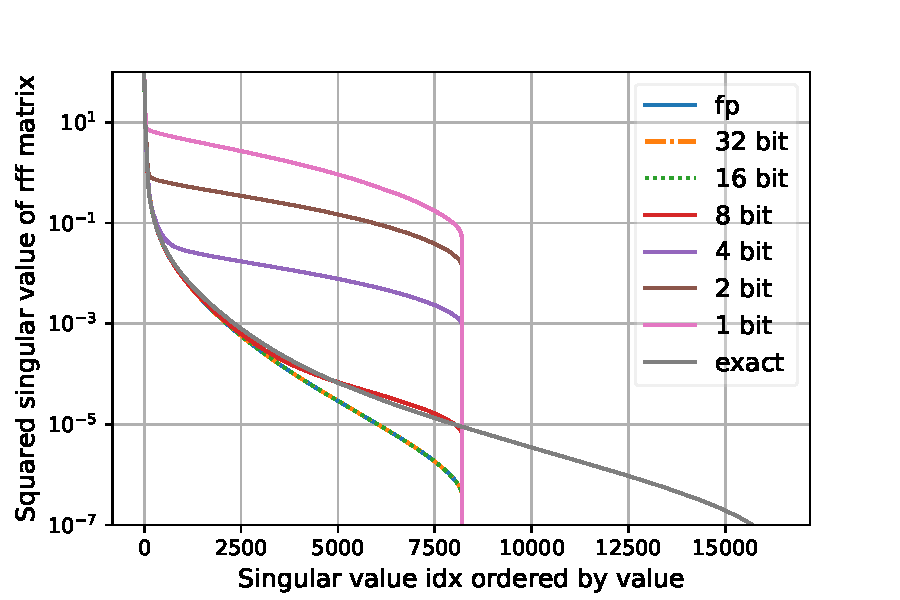
\includegraphics[width=.45\linewidth]{figures/spectrum_n_rff_8192.pdf} &
		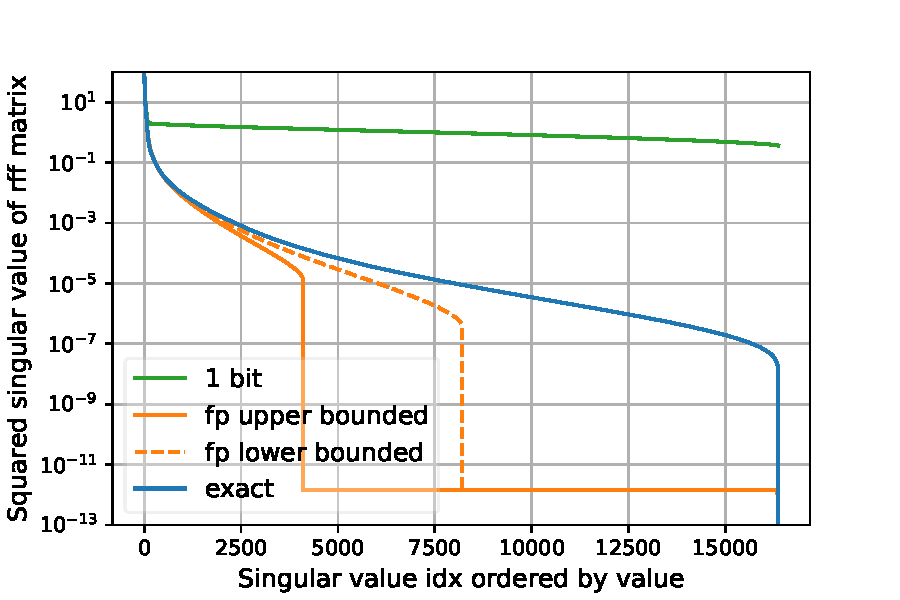
\includegraphics[width=.45\linewidth]{figures/different_spectrum_with_same_kernel_approx_error_log.pdf} \\
%		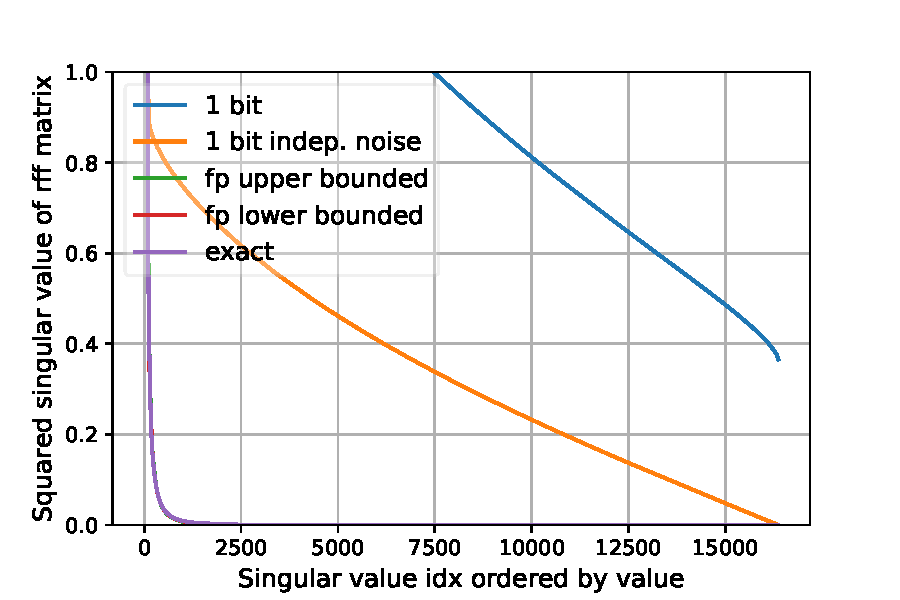
\includegraphics[width=.33\linewidth]{figures/different_spectrum_with_same_kernel_approx_error.pdf}\\
		(a) & (b) %& (c)
	\end{tabular}
	\caption{Spectrum (eigen values) of the kernel matrix. (a) The spectrums from different precision representation is shown under 8192 random Fourier features. (b) Configurations with similar approximation errors can demonstrate very different spectrum; we compare the 1 bit representation to the full precision configurations giving 1) the highest approx. error that is lower than the 1 bit configuration 2) the lowest approx. error that is higher than the 1bit configuration.}
	\label{fig:spectrums}
\end{figure}

In our theory in Section~\ref{sec:elevate_spectrum}, we have been discussing how low precision introduce quantization variance, which results in bumping up the spectrum of kernel matrix. In Figure~\ref{fig:spectrums} (a), we demonstrate the kernel matrix spectrum from 8192 random Fourier features in different precision. 
We can observe 8, 16 and 32 bits representation has spectrums close to the spectrum of full precision RFF kernel matrix. However, for 4, 2 and 1 bits representation has significantly higher spectrums than 8, 16 and 32 bits representation. Remember that in Figure~\ref{fig:kernel_and_l2}, we have seen 8, 16 and 32 bits representation demonstrates similar l2 loss, while 4, 2 and 1 bits can show observably worse performance. \emph{From these observations, we believe spectrum is closely correlated with the validation l2 loss. Indeed if the two RFF kernel matrices has the same spectrum, the RFF features matrices are only different up to rotation and flipping; it is the sole quantity to decide the behavior of a kernel regression model.} 

Additionally, we compare to the correlation between kernel approximation error and l2 loss, to further emphasize the strong correlation between spectrum and l2 loss. In Figure~\ref{fig:spectrums} (b), we demonstrates the spectrums from 3 configurations with very similar kernel approximation error. Specifically, we compare 1 bit RFF with 131k features to two full precision RFF configuration with the closest kernel approximation error; these 2 full precision configurations respectively gives 1) the highest approx. error that is lower than the 1 bit configuration (8192 features) 2) the lowest approx. error that is higher than the 1bit configuration (4096 features). The 3 configurations shows close relative kernel approximation error around $1e^{-2}$, but can demonstrate very different spectrum in Figure~\ref{fig:spectrums} and very different validation l2 loss in Figure~\ref{fig:kernel_and_l2} (d).

\begin{figure}
	\centering
	\begin{tabular}{c c}
		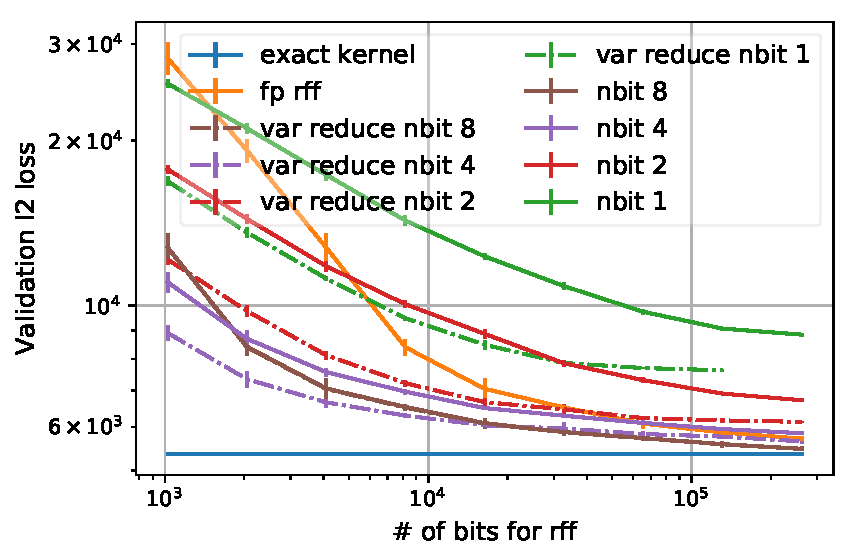
\includegraphics[width=.45\linewidth]{figures/valid_l2_var_reduction.pdf} &
		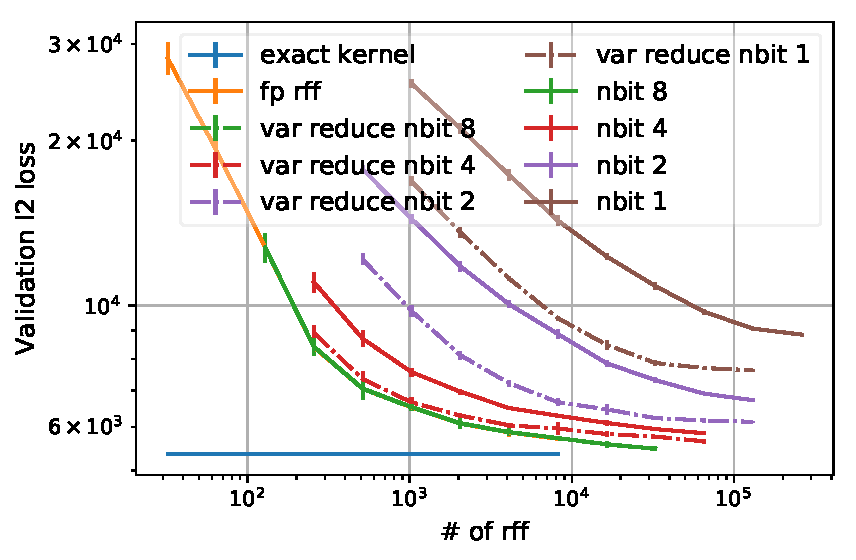
\includegraphics[width=.45\linewidth]{figures/valid_l2_n_fp_var_reduction.pdf} \\
		(a) & (b)
	\end{tabular}
	\caption{We train with low precision rffs and test with full precision rffs. Though the model is trained with low precision features, the test l2 loss can be improved by reducing variance in test rffs. (a) compare different precision representation under same memory bits budgets. (b) compare different precision representation with the same number of random Fourier features.}
	\label{fig:var_reduction}
\end{figure}


\begin{figure}
	\centering
	\begin{tabular}{c c}
		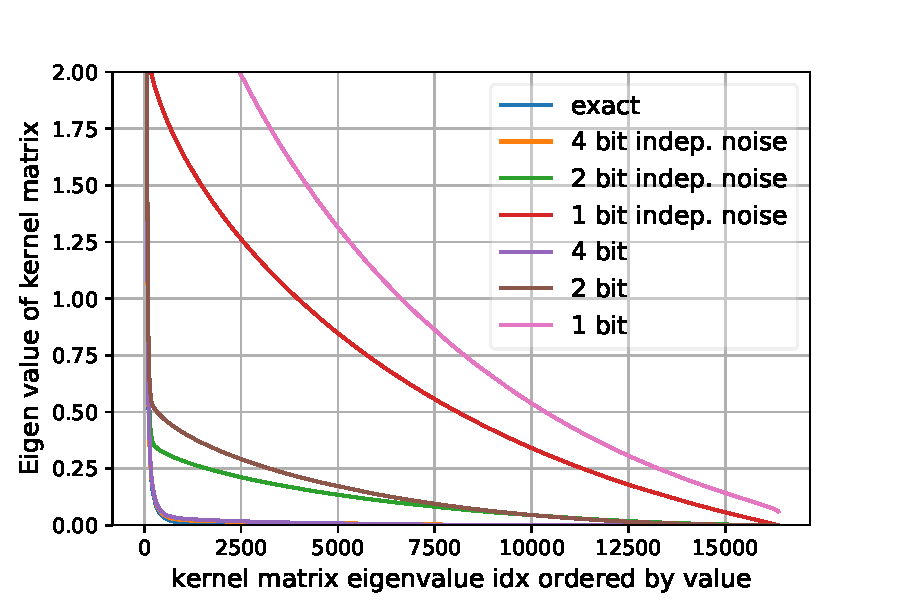
\includegraphics[width=.45\linewidth]{figures/spectrum_1024_indep.pdf} &
		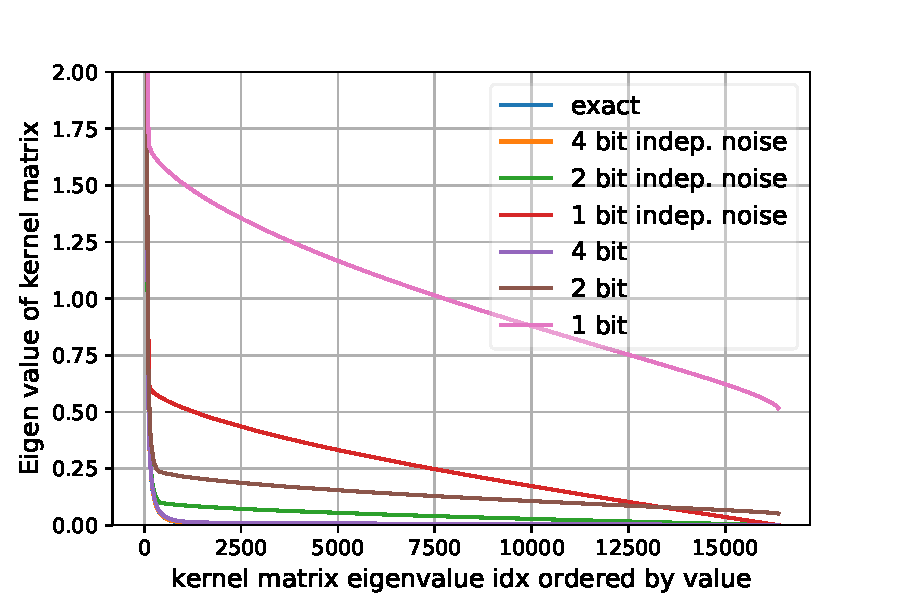
\includegraphics[width=.45\linewidth]{figures/spectrum_8192_indep.pdf} \\
		(a) & (b) \\
		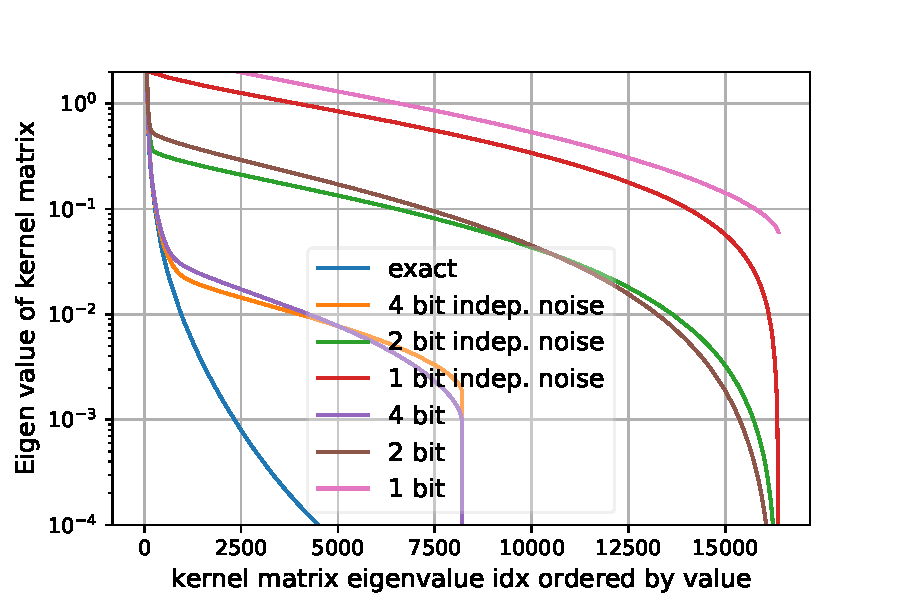
\includegraphics[width=.45\linewidth]{figures/spectrum_1024_indep_log.pdf} &
		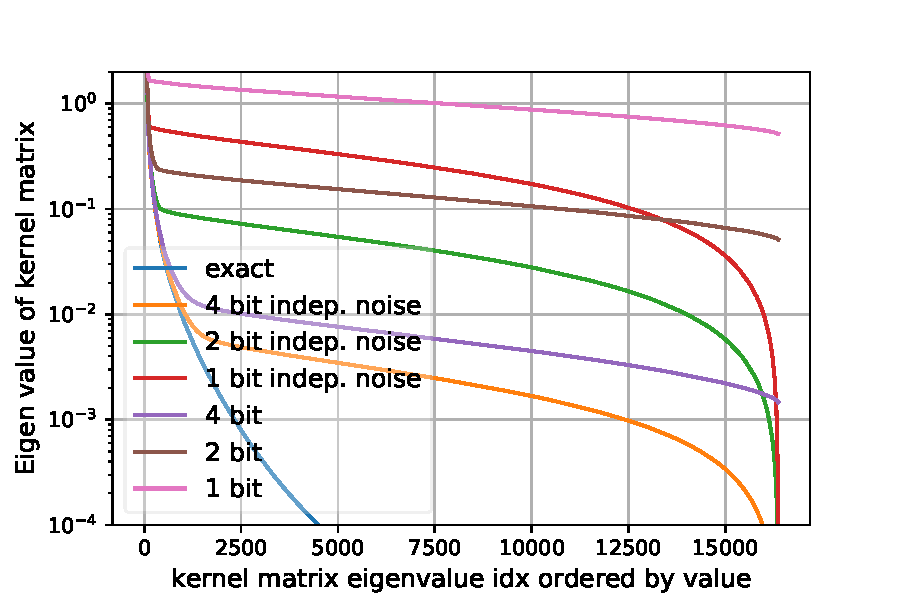
\includegraphics[width=.45\linewidth]{figures/spectrum_8192_indep_log.pdf} \\
		(c) & (d)
	\end{tabular}
	\caption{Spectrum (eigen values) of the kernel matrix. (a) The spectrum from different precision representation under 3.2k bits memory budget (1024 full precision rffs) for the feature of each sample. (b) The spectrum from different precision representation under 25.6k bits memory budget (1024 full precision rffs) for the feature of each sample.}
\end{figure}

%
%512 2 bits, 4096 fp 8192 fp, 4096 1 bit

